\documentclass{article}
\usepackage{listings, verbatim}
\usepackage[usenames,dvipsnames]{color}
\usepackage[usenames,dvipsnames,svgnames,table]{xcolor}
\usepackage{amsmath,amsfonts,graphicx,comment,typearea,amsthm,subcaption}
\usepackage{xcomment,psfrag,enumerate,scrpage2,xspace,hyperref,rotating,float}
\usepackage[top=1in, bottom=1.25in, left=1.25in, right=1.25in]{geometry}

\begin{document}

\title{MAS8381: Marketing Data Project}
\author{Michael Dunne-Willows: 120065714\\
Antonia Kontaratou: 150469832\\
Hayley Moore: 110331287}
\maketitle

\section{Converting the Variables}
We started our analysis by deciding whether a variable should be converted into a factor. We decided that if the variable was categorical, only had a small number of values and was unordered then to convert the variable to a factor. Table~\ref{variables} shows the variables an whether they are used as a factor or not.
\begin{table}[H]
\centering
\begin{tabular}{|l|l|l|}
\hline
\textbf{Variable} &\textbf{Used as} &\textbf{Levels/definition}\\
\hline
Income       &Continuous variable  & Annual household income\\
\hline
Sex          &Factor with 2 levels &1. Male \\
&&2. Female\\
\hline
Marital      &Factor with 5 levels &1. Married \\
&&2. Living together, not married \\
&&3. Divorced or separated \\
&&4. Widowed \\
&&5. Single, never married\\
\hline
Age          &Continuous variable  &Age of person answering the questionnaire\\
\hline
Edu          &Factor with 6 levels &1. Grade 8 or less \\
&&2. Grades 9 to 11 \\
&&3. Graduated high school \\
&&4. 1 to 3 years of college \\
&&5. College graduate \\
&&6. Grad Study\\
\hline
Occupation   &Factor with 9  &1. Professional/Managerial \\
&&2. Sales Worker \\
&&3. Factory Worker/Laborer/Driver \\
&&4. Clerical/Service Worker \\
&&5. Homemaker \\
&&6. Student, HS or College \\
&&7. Military \\
&&8. Retired \\
&&9. Unemployed\\
\hline
Lived        &Factor with 5 levels &1. Less than one year \\
&&2. One to three years \\
&&3. Four to six years \\
&&4. Seven to ten years \\
&&5. More than ten years\\
\hline
Dual\_Income &Factor with 3 levels &1. Not Married \\
&&2. Yes \\
&&3. No\\
\hline
Household    &Continuous variable  &Number of people living in the house\\
\hline
\end{tabular}
\end{table}
\begin{table}[H]
\centering
\begin{tabular}{|l|l|l|}
\hline
Householdu18 &Continuous variable  &Number of under 18's living in the house\\
\hline
Status       &Factor with 3 levels &1. Own \\
&&2. Rent \\
&&3. Live with Parents/Family\\
\hline
Home\_Type   &Factor with 5 levels &1. House \\
&&2. Condominium \\
&&3. Apartment \\
&&4. Mobile Home \\
&&5. Other\\
\hline
Ethnic       &Factor with 8 levels &1. American Indian \\
&&2. Asian \\
&&3. Black \\
&&4. East Indian \\
&&5. Hispanic \\
&&6. Pacific Islander \\
&&7. White \\
&&8. Other\\
\hline
Language     &Factor with 3 levels &1. English \\
&&2. Spanish \\
&&3. Other\\
\hline
\end{tabular}
\caption{variables}
\label{variables}
\end{table}

\noindent We had to just our judgement to set \textsf{Edu} and \textsf{Lived} as a factor as they were both ordered categorical variables. We decided that they should be classed as factors since in the case of education the gaps between levels were not consistent.
\\\\
We also decided that \textsf{Household} and \textsf{Householdu18} should be used as continuous variables since the gaps between each level were consistent this time. For example looking at the \textsf{Householdu18} information below
\begin{verbatim}
Householdu18 : PERSONS IN HOUSEHOLD UNDER 18 
0. None 1. One 2. Two 3. Three 4. Four 5. Five 6. Six 7. Seven 
8. Eight 9. Nine or more
\end{verbatim}
we can see that each gap is equivalent to one more under 18 person living in the house.



\section{Handling Missing Data}

\label{handling}
Upon first inspection of the data we see there are many missing values. This is common in datasets and can be the result of many situations- within surveys, for example, participants may have refrained from answering certain questions or stopped participating part way through a long term study into the impact of, say a new medicine. 
Missing data becomes a serious problem, however when we wish to make inferences by fitting models to the full data set and we need meaning full values in every cell of our database. 

\subsection{Omitting missing data}
The quickest way to solve the missing data problem is to omit every observation where at least one variable has a missing value.  

\begin{verbatim}  
marketing = na.omit(marketing)  
\end{verbatim}
The simplicity of this method comes a price because we lose all the information contained in any of the other variables for an observation which carries even a single missing value.


\begin{verbatim}
> sum(is.na(marketing))/dim(marketing)[1]
[1] 0.2995663
\end{verbatim}
In the case of our marketing dataset there are approximately 2600 such observations which make up about 30\% of the data. Losing so much of our data would have a significant impact on the validity of any fitted models. We need a more preservative way to deal with the missing values.

\subsection{Replacing with the predictor mode}
It is common practice when dealing with missing data to replace missing values with the mean value of the variable in question. For categorical data, such as that in our marketing data, the mode of the data performs similarly. Note that we must not fill-in/impute any values for 'Income' as this is our response variable.
The following function can be called on our marketing data set to carry out the necessary substitutions. The mode function involved has been written separately as this is not included in R by default.

{\small
\begin{verbatim}
NA_to_mode = function(m){
  for ( i in 2:14) {
    m[,i][is.na(m[,i])] = Mode(na.omit(m)[,i])
  }
  return(m)
}
\end{verbatim}
}
This method has the major advantage over the latter in that we dont't lose any of the information stored in data values adjacent to missing data. Implementing this method does not require a significant amount of computing time in the case of our dataset.
\\\\
One potential flaw in this method is that all the missing values of a variable will be given the same value. The reason these data are missing may be significant, e.g. members of a given ethnic background may have been generally reluctant to divulge said information to a survey, this may have resulted in the majority of missing 'Ethnic' values actually belonging to people of the same given ethnicity which, crucially would not be reflected in the mode of the available “Ethnic” values.


\subsection{Multiple Imputation}
To combat this potential bias, we can look at the available data fo the observations in question and base our imputations on them. For this method we will make use of the CRAN Package “mice”. This package can implement multiple techniques to predict data values depending on whether they are ordered/unordered categorical or continuous etc. Once we specify these methods, we can run the  following command to perform several iterations of these methods of imputation and finally update our marketing dataset with the new complete dataset.
{\small
\begin{verbatim}
data(marketing)
result = (mice(marketing, m =5, me = method))
\end{verbatim}

\begin{verbatim}
marketing = complete(result,1)
\end{verbatim}
}
\noindent Despite the extra computation time, this method of multiple imputation is the best of the three we have investigated because it neither removes valuable information from the data nor does it assign the same value to each missing value of a given variable regardless of the available adjacent data.
\\\\
Having decided on our imputation method, we are now in a position to proceed to fit various models to the data with the aim of inferring which of our predictors best predict the value of `Income'. We decide to make one last check before proceeding- to see how much of the data for each predictor we have actually imputed. This is shown in Figure~\ref{Proportion}
\\\\
One value catches our attention- the predictor `Lived' has required $10\%$ of it's data to imputed. This may reflect badly on any apparent significance to this predictor later in our analysis.
\begin{figure}[h!]
  \centering
  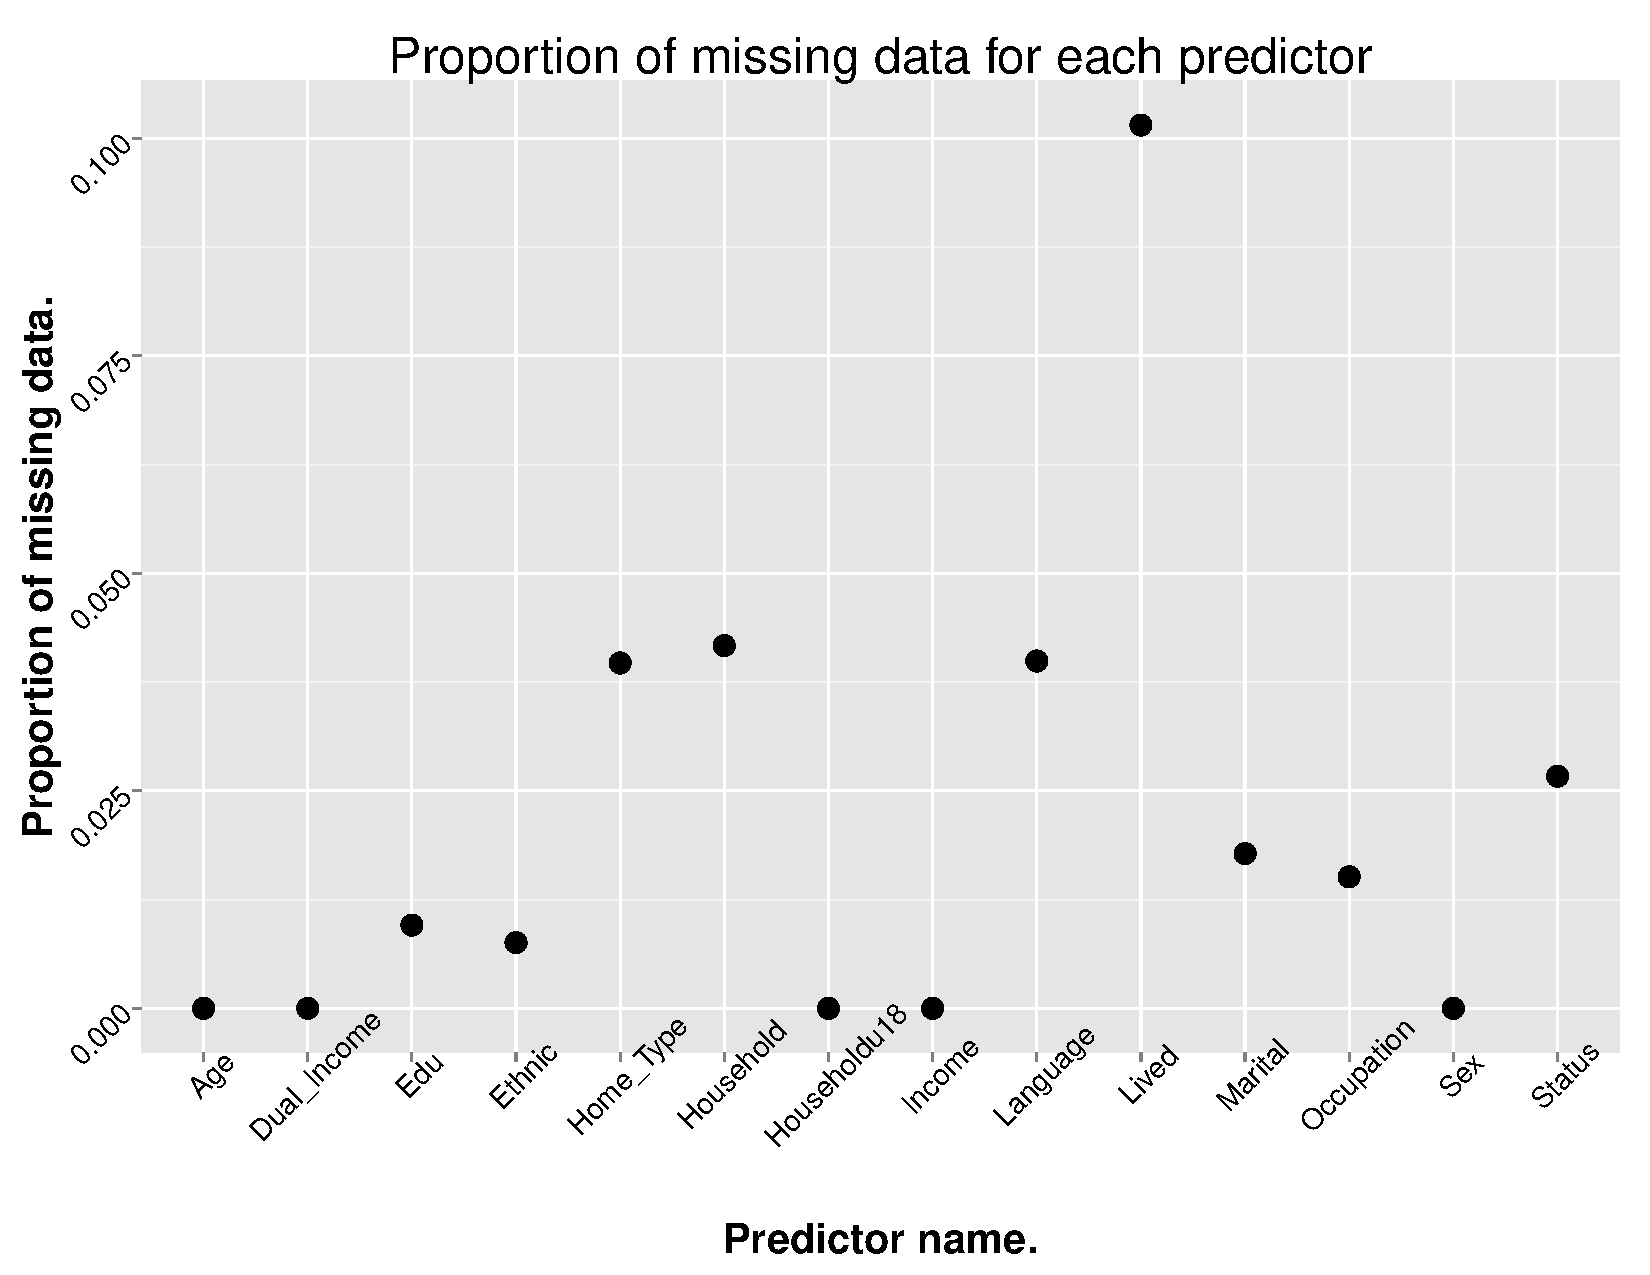
\includegraphics[width=0.7\textwidth]{HandlingMissingData/PropMissingData.pdf}
  \caption{Proportion of Missing Data.}
  \label{Proportion}
\end{figure}


\section{Frequentest Linear Model }
\subsection{Linear Model Selection and Regularization}  
The concept of the Linear Model Selection and Regularization is to improve the linear model by replacing the plain least squares fitting with an alternative fitting procedure that might lose a little bit of fitting but yields better predictive performance and model interpretability. 
\\\\
The relative approaches that follow are the Subset Selection and the Shrinkage. The first, involves identifying a subset of p predictors that we believe to be related to the response and then fitting the model using least squares on the reduced set of variables. The second, involves fitting the model using all p predictors but the coefficients are shrunken towards zero (or exactly zero depending on the method used) relative to the least squares estimates, in order to reduce the variance. From the first category we will use the Best Subset Selection and from the second the Lasso.

\subsection{Best Subset Selection}

In the Best Subset Selection we begin by fitting all p models $\binom{p}{2}$ models that contain exactly one predictor, all $\binom{p}{2} =\frac{p(p-1)}2$ models that contain exactly two predictors and so forth and finally we look at the resulting models and try to identify the best model.
\\\\
In our example the initial marketing data contain 13 predictors and the response, after the factorizing we get 42 variables and the intercept. After fitting the model using Best Subset Selection for various numbers of variables we observed that the indicators that we examine in this method, the adjusted R, the BIC and the Cp suggested that we use more variables to fit the model. To be more precise the more variables added, the best the indicators turned out to be. So for model simplicity and in order to avoid over-fitting, we decided to use the first 13 variables that are considered the most important by the model(the model uses the lowest RSS as criteria). In the text below we can see which predictors are considered to be the most important according to the Best Subset Solution.

{\small
\begin{verbatim}
          Sex2 Marital2 Marital3 Marital4 Marital5 Age Edu2 Edu3 Edu4

13  ( 1 ) " "  " "      " "      " "      " "      "*" " "  "*"  "*" 
          Edu5 Edu6 Occupation2 Occupation3 Occupation4 Occupation5
      
13  ( 1 ) "*"  "*"  " "         " "         "*"         " "        
          Occupation6 Occupation7 Occupation8 Occupation9 Lived2 Lived3

13  ( 1 ) "*"         " "         "*"         "*"         " "    " "   
          Lived4 Lived5 Dual_Income2 Dual_Income3 Household Householdu18
      
13  ( 1 ) " "    " "    "*"          "*"          " "       " "         
          Status2 Status3 Home_Type2 Home_Type3 Home_Type4 Home_Type5
   
13  ( 1 ) "*"     "*"     " "        " "        " "        " "       
          Ethnic2 Ethnic3 Ethnic4 Ethnic5 Ethnic6 Ethnic7 Ethnic8
 
13  ( 1 ) " "     " "     " "     " "     " "     " "     " "    
          Language2 Language3
    
13  ( 1 ) " "       " " 
\end{verbatim}
}
\noindent Let Y indicate the response which in our case is the income. Then the model according to the Best Subset Selection will be:
\\\\
$Y= \beta+0$ + $\beta_1$Age + $\beta_2$Edu3 + $\beta_3$Edu4 + $\beta_4$Edu5 + $\beta_5$Edu6 + $\beta_6$Occupation4 + $\beta_7$Occupation6 + $\beta_8$Occupation8 + $\beta_9$Occupation9 + $\beta_10$Dual\_Income2+ $\beta_11$Dual\_Income3 + $\beta_12$Status2 + $\beta_13$Status3
\\\\
We conclude that income is influenced by the Age and the level of education and more precisely by the higher levels of education. Furthermore it is affected by the two most extreme occupation categories, the Clerical/Service Worker and the unemployed as well as the Students and the retired. The dual income is an other factor that affects our response and the status of the householder as well and more specifically the factors related to the fact that the householder might be paying a rent or living with his parents/family. 
\\\\
Below we can also see how the $R^2$ is formulated while adding more variables.
{\small
\begin{verbatim}
[1] 0.1754538 0.2667926 0.3102752 0.3386352 0.3570837 0.3771129 0.3958195 0.4064571
[9] 0.4164211 0.4221043 0.4276303 0.4322475 0.4365138
 \end{verbatim}
 }
\noindent We see that the $R^2$ statistics increases from 17.55\% when only 1 variable is included in the model to 43.65\% when we use 13 variables, which means that  the model explains 43.65\% of the variability of the response data around its mean when we use these 13 predictors.
\\\\
The next step is to see the plots produced for RSS, adjusted $R^2$ , Cp and BIC, shown in Figure~\ref{RSS}.
\begin{figure}[h]
    \centering
    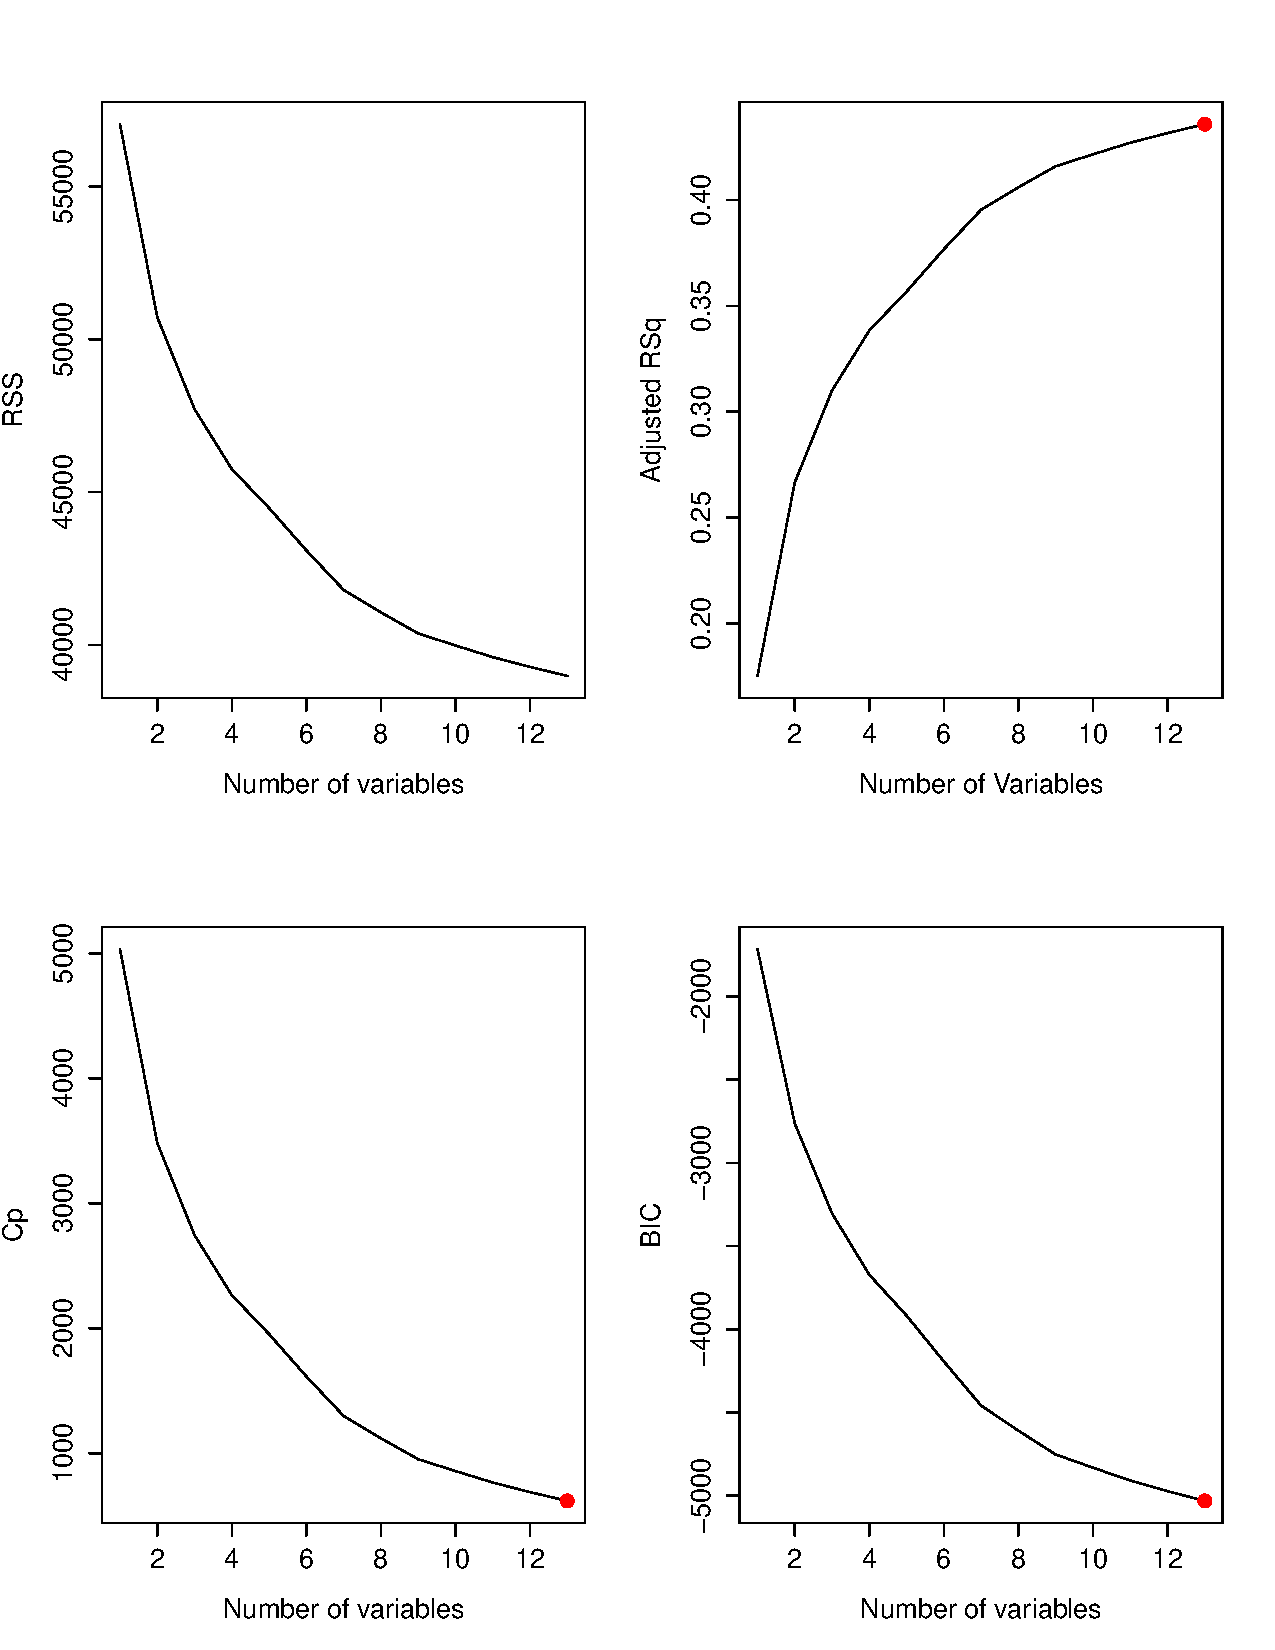
\includegraphics[width = 0.55\textwidth]{RSS_ETC_PLOT.pdf}
    \caption{Plots of RSS, adjusted $R^2$, Cp and BIC} 
    \label{RSS}
\end{figure} 
If we use BIC as the selection criteria, it is suggested that we use a subset of thirteen predictors(as expected) that are believed to be related to the response as BIC reaches its lowest value when it uses thirteen predictors. To see which thirteen predictors we plot the BIC and get the following figure that results to the model mentioned previously.
\begin{figure}[h]
    \centering
    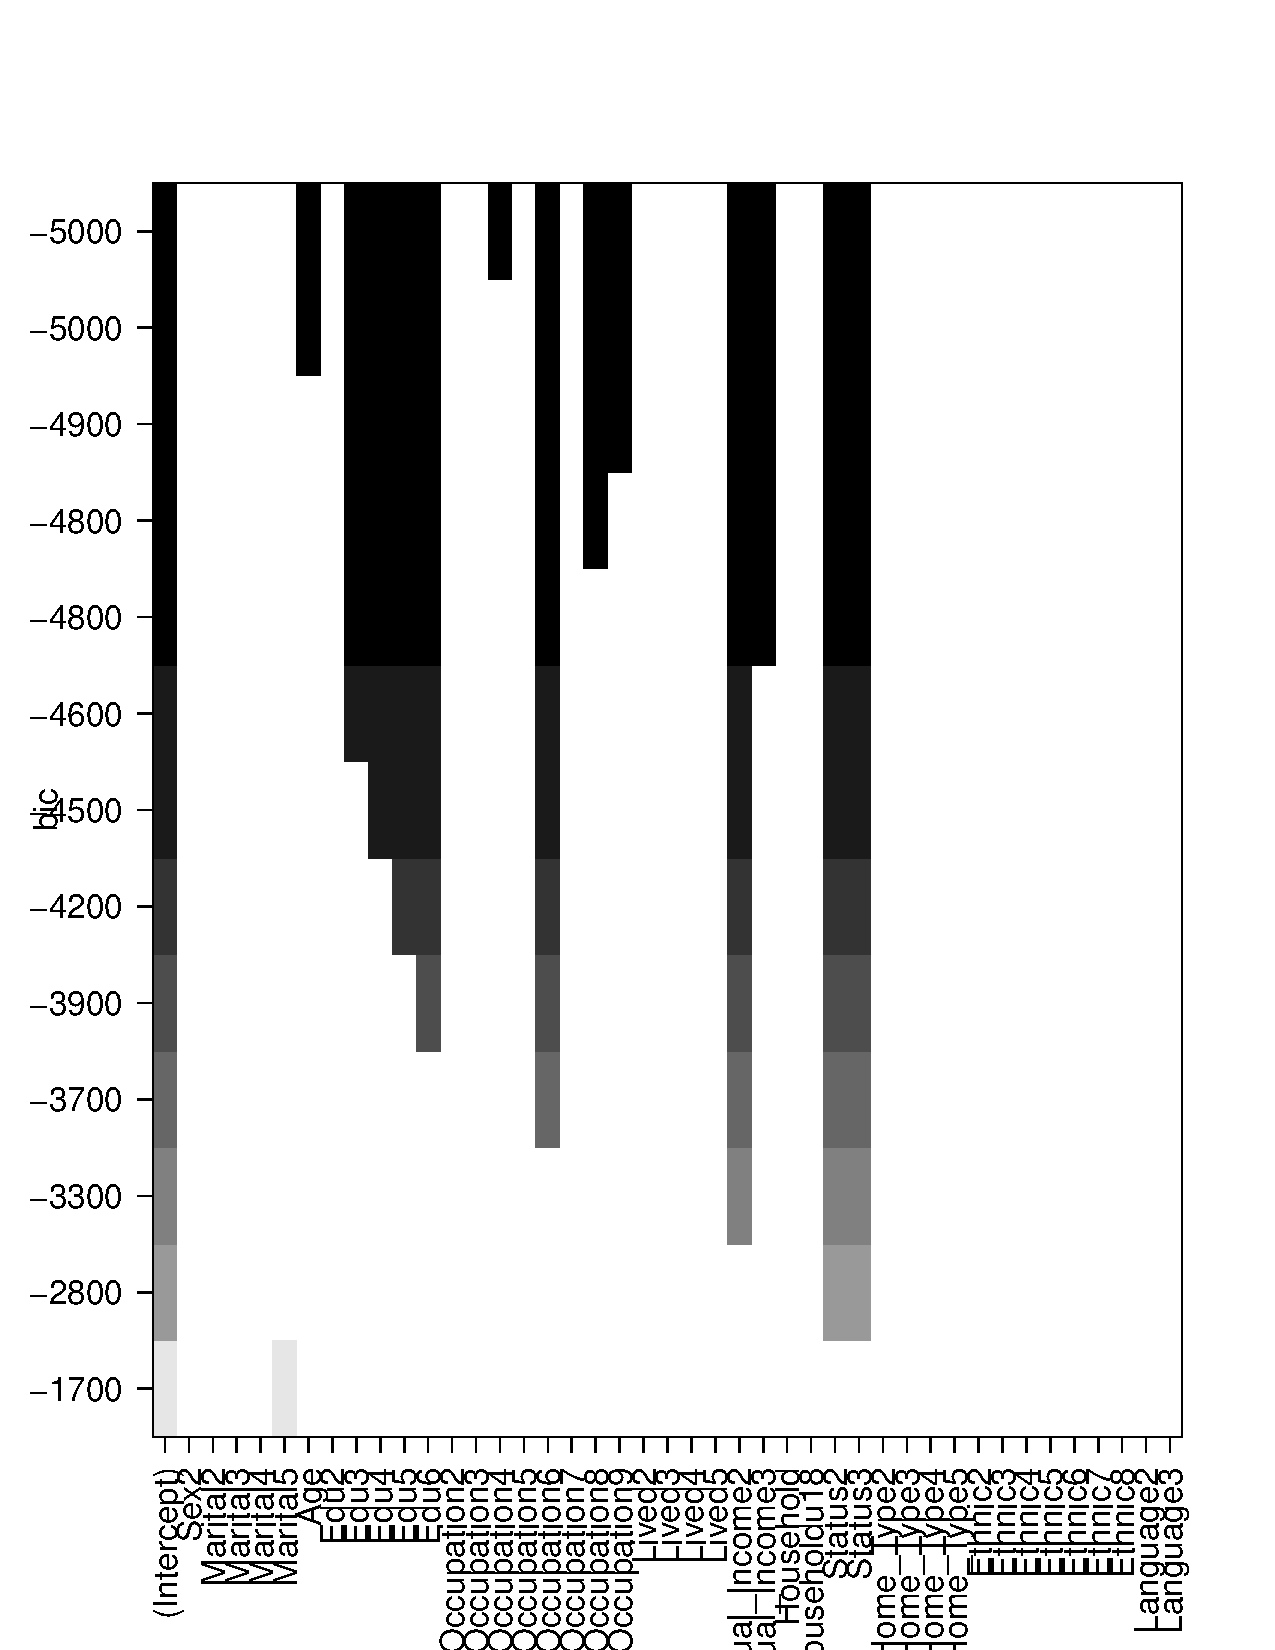
\includegraphics[scale=0.3]{BIC_PLOT.pdf}
    \caption{Selected variables for the best model ranked according to BIC}
    \label{BIC}
\end{figure}
The disadvantage of the above indicators (including BIC) is that they all adjust the training error, so in the next part we are going to use the cross validation that estimates the test error directly.

\subsection{Cross Validation}
We are interested in the test error which is the average error that results from using a statistical learning method to predict a response on a new observation, which means a measurement that was not used in training the method. 
\\\\
So we use the cross validation which is a method that estimates the test error holding out a subset  of the training observations from the fitting process and then applying the statistical learning method to those held out observations. Again for model simplicity we choose to use up to 13 variables to the resulting model because the more variables we added the lowest the test MSE was getting.
\\\\
\begin{figure}[H]
    \centering
   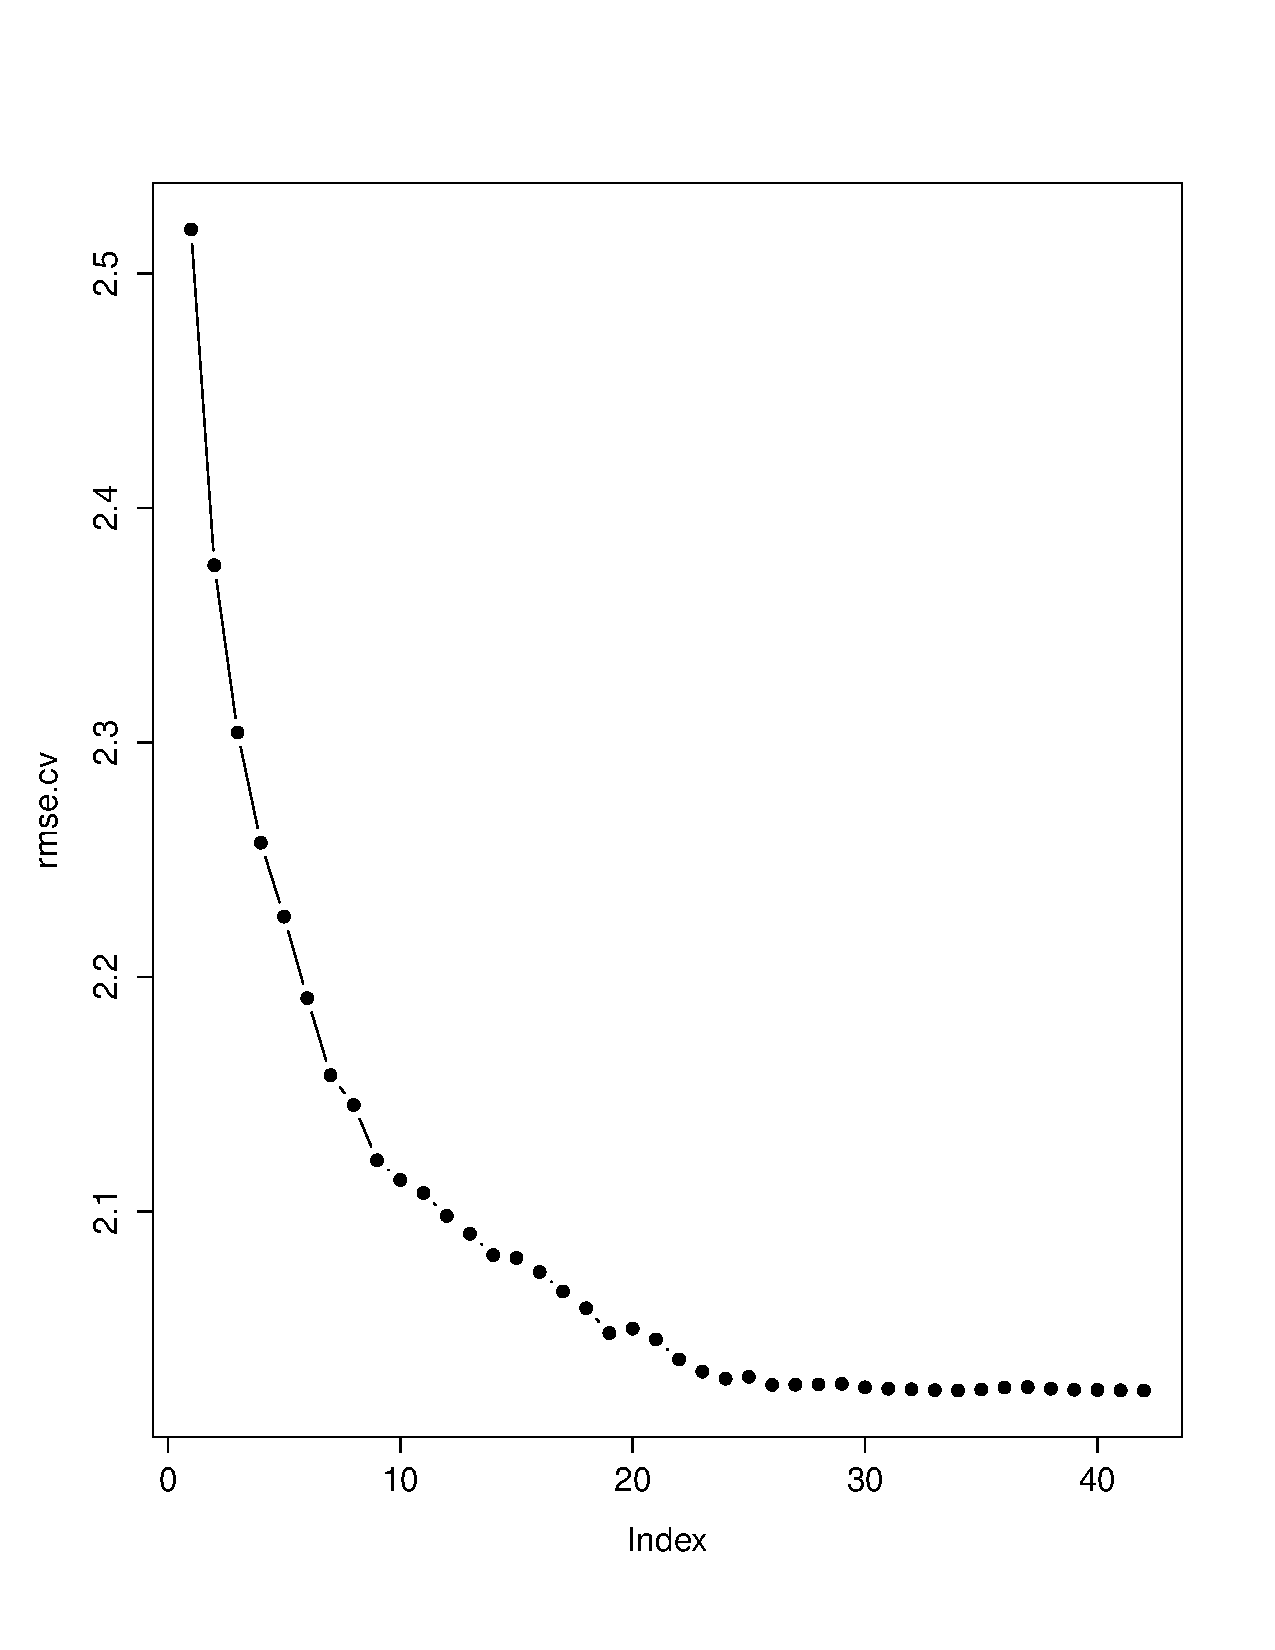
\includegraphics[scale=0.3]{CROSS_VALIDATION_MSE_PLOT.pdf}
    \caption{Cross validation error}
    \label{CrossValidationError}
\end{figure}
\noindent From which we can see that cross-validation selects a 13 variable model with coefficients:
{\small
\begin{verbatim}
 (Intercept)          Age         Edu3         Edu4         Edu5 
   3.5684152    0.2091928    0.9963787    1.5503228    2.2064117 
        Edu6  Occupation4  Occupation6  Occupation8  Occupation9 
   2.5584260   -0.5856842   -1.2213397   -1.5116519   -1.1271196 
Dual_Income2 Dual_Income3      Status2      Status3 
   1.3589114    0.8069902   -1.4836791   -0.8627755 
 \end{verbatim}
 }
\noindent The above coefficients constitute the coefficients of the model mentioned in the previous section.

\subsection{The lasso}
Unlike Best Subset Selection presented in a previous subsection the Lasso includes all p predictors and uses a penalty depending on the tuning parameter $\lambda$ to perform a variable selection by shrinking the coefficients to zero if $\lambda$ is sufficiently large.
\\\\
In the Lasso the best $\lambda$ is selected according to the variable which presents the lowest error, but we selected a $\lambda$ = 0.3 as we did not want to have more than approximately 11 variables and the intercept to avoid over-fitting. As it expected the more variables added, the less the test error but in our example the higher value of lambda selected did not affect the corresponding test in an important way.
\begin{center}
\begin{minipage}[c]{0.4\textwidth}
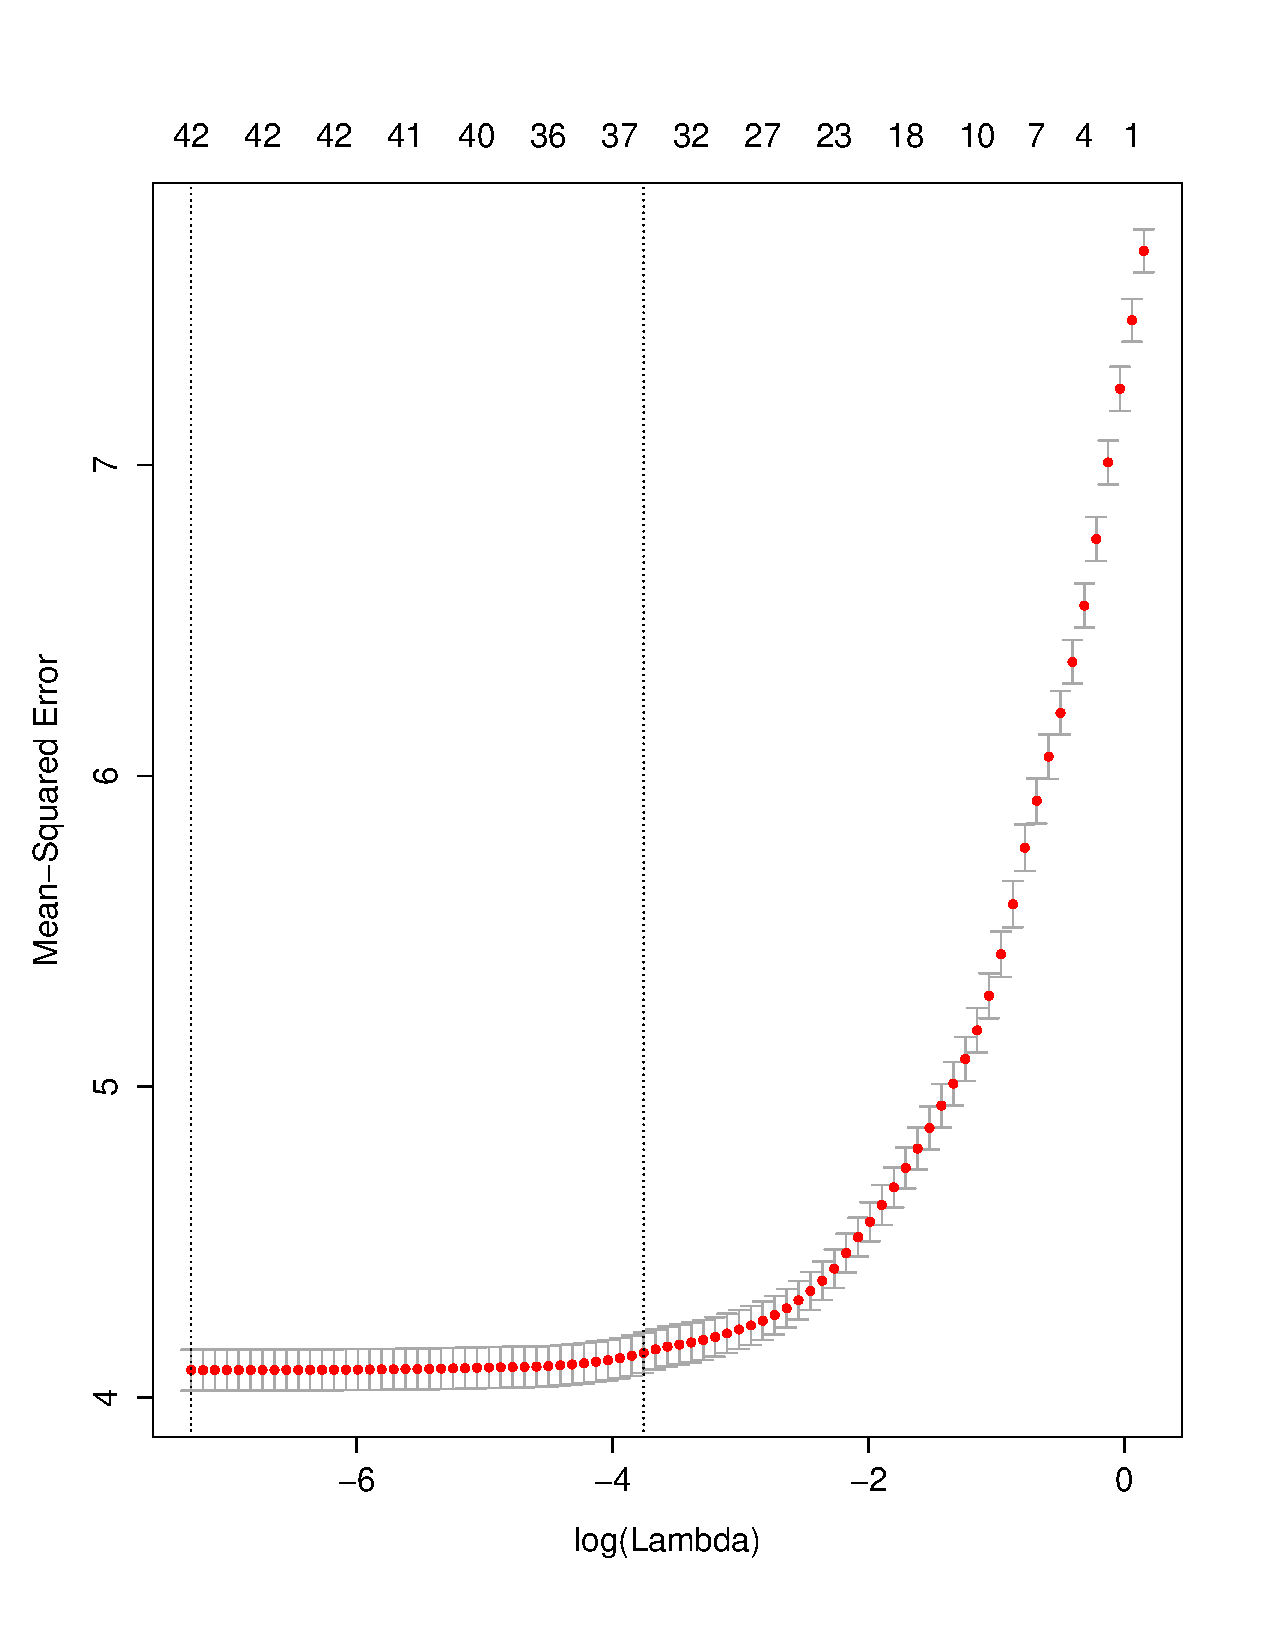
\includegraphics[width = \textwidth]{LASSO_ERROR_PLOT.pdf}
\end{minipage}\quad\quad\quad
\begin{minipage}[c]{0.4\textwidth}
\textbf{Lasso Coefficients}
{\small
\begin{verbatim}
(Intercept)   4.93382364      
Marital5     -0.49340288
Age           0.11818877
Edu2         -0.58760282      
Edu5          0.33818740
Edu6          0.65078190       
Occupation6  -0.82120634    
Dual_Income2  0.83935922     
Status2      -0.47429447
Status3      -0.49832197       
Home_Type3   -0.21073592      
Ethnic5      -0.02600054
\end{verbatim}
}
\end{minipage}
\end{center}
The model to which we conclude using the Lasso is slightly different from the one that we got from the Best Subset Selection. Now the 11 variables suggested to be used to fit the model are: the marital status and especially the fact that someone is single as opposed to all the other factors of this variable, the age, the fact that someone is either a college or a university graduate or at Grades 9 to 11. Besides the existence of a dual income and the facts that someone might pay a rent or live with his family affect the Income as well. Some other factors that appear in this model is the home type and the ethnicity that are negatively correlated with our response which means that if someone stays in an apartment or has a Hispanic ethnicity it is more probable that his income is less as opposed to the other factors of the corresponding variables.






\section{Bayesian Analysis}
We used RJAGS in our Bayesian analysis. RJAGS is a way of calling JAGS from with in \textsf{R}. JAGS is a program for the statistical analysis of Bayesian models by Markov Chain Monte Carlo, MCMC. MCMC is a way of sampling form a distribution by using a Markov chain with its equilibrium distribution the same as the distribution we wish to sample from. A MCMC has two stages a burn in stage, where the Markov chain hasn't reached equilibrium, and a converged stange, where the chain has reached equilibrium.
\\\\
When using \textsf{R} it calls $\beta_0$ beta[1].
\subsection{Saturated Model}
We start the Bayesian analysis by modelling the saturated model with the missing data handled by just simply omitting it, later on we use the mice method mentioned earlier to handle the missing values. We have chosen to use a vague prior on each of our parameters, $\beta_i$, and for the precision, $\tau$. The model string  for this is 
{\small
\begin{verbatim}
modelstring = "
model {
for (i in 1:n) {
mean[i] =  inprod(X[i,],beta)
y[i]~dnorm(mean[i],tau)
}
for (j in 1:p) {
beta[j]~dnorm(0,0.001)
}
tau~dgamma(1,0.001)
}
"
\end{verbatim}
}
\noindent The MCMC had a burn in of 1000 iterations and a run of 10,000 iterations. From the plots of $\beta_1$ to $\beta_4$ we can see that the distribution converged. This is shown in Figure~\ref{saturated_beta1-4} by the "furry caterpillar" effect we see.
\begin{figure}[h!]
\centering
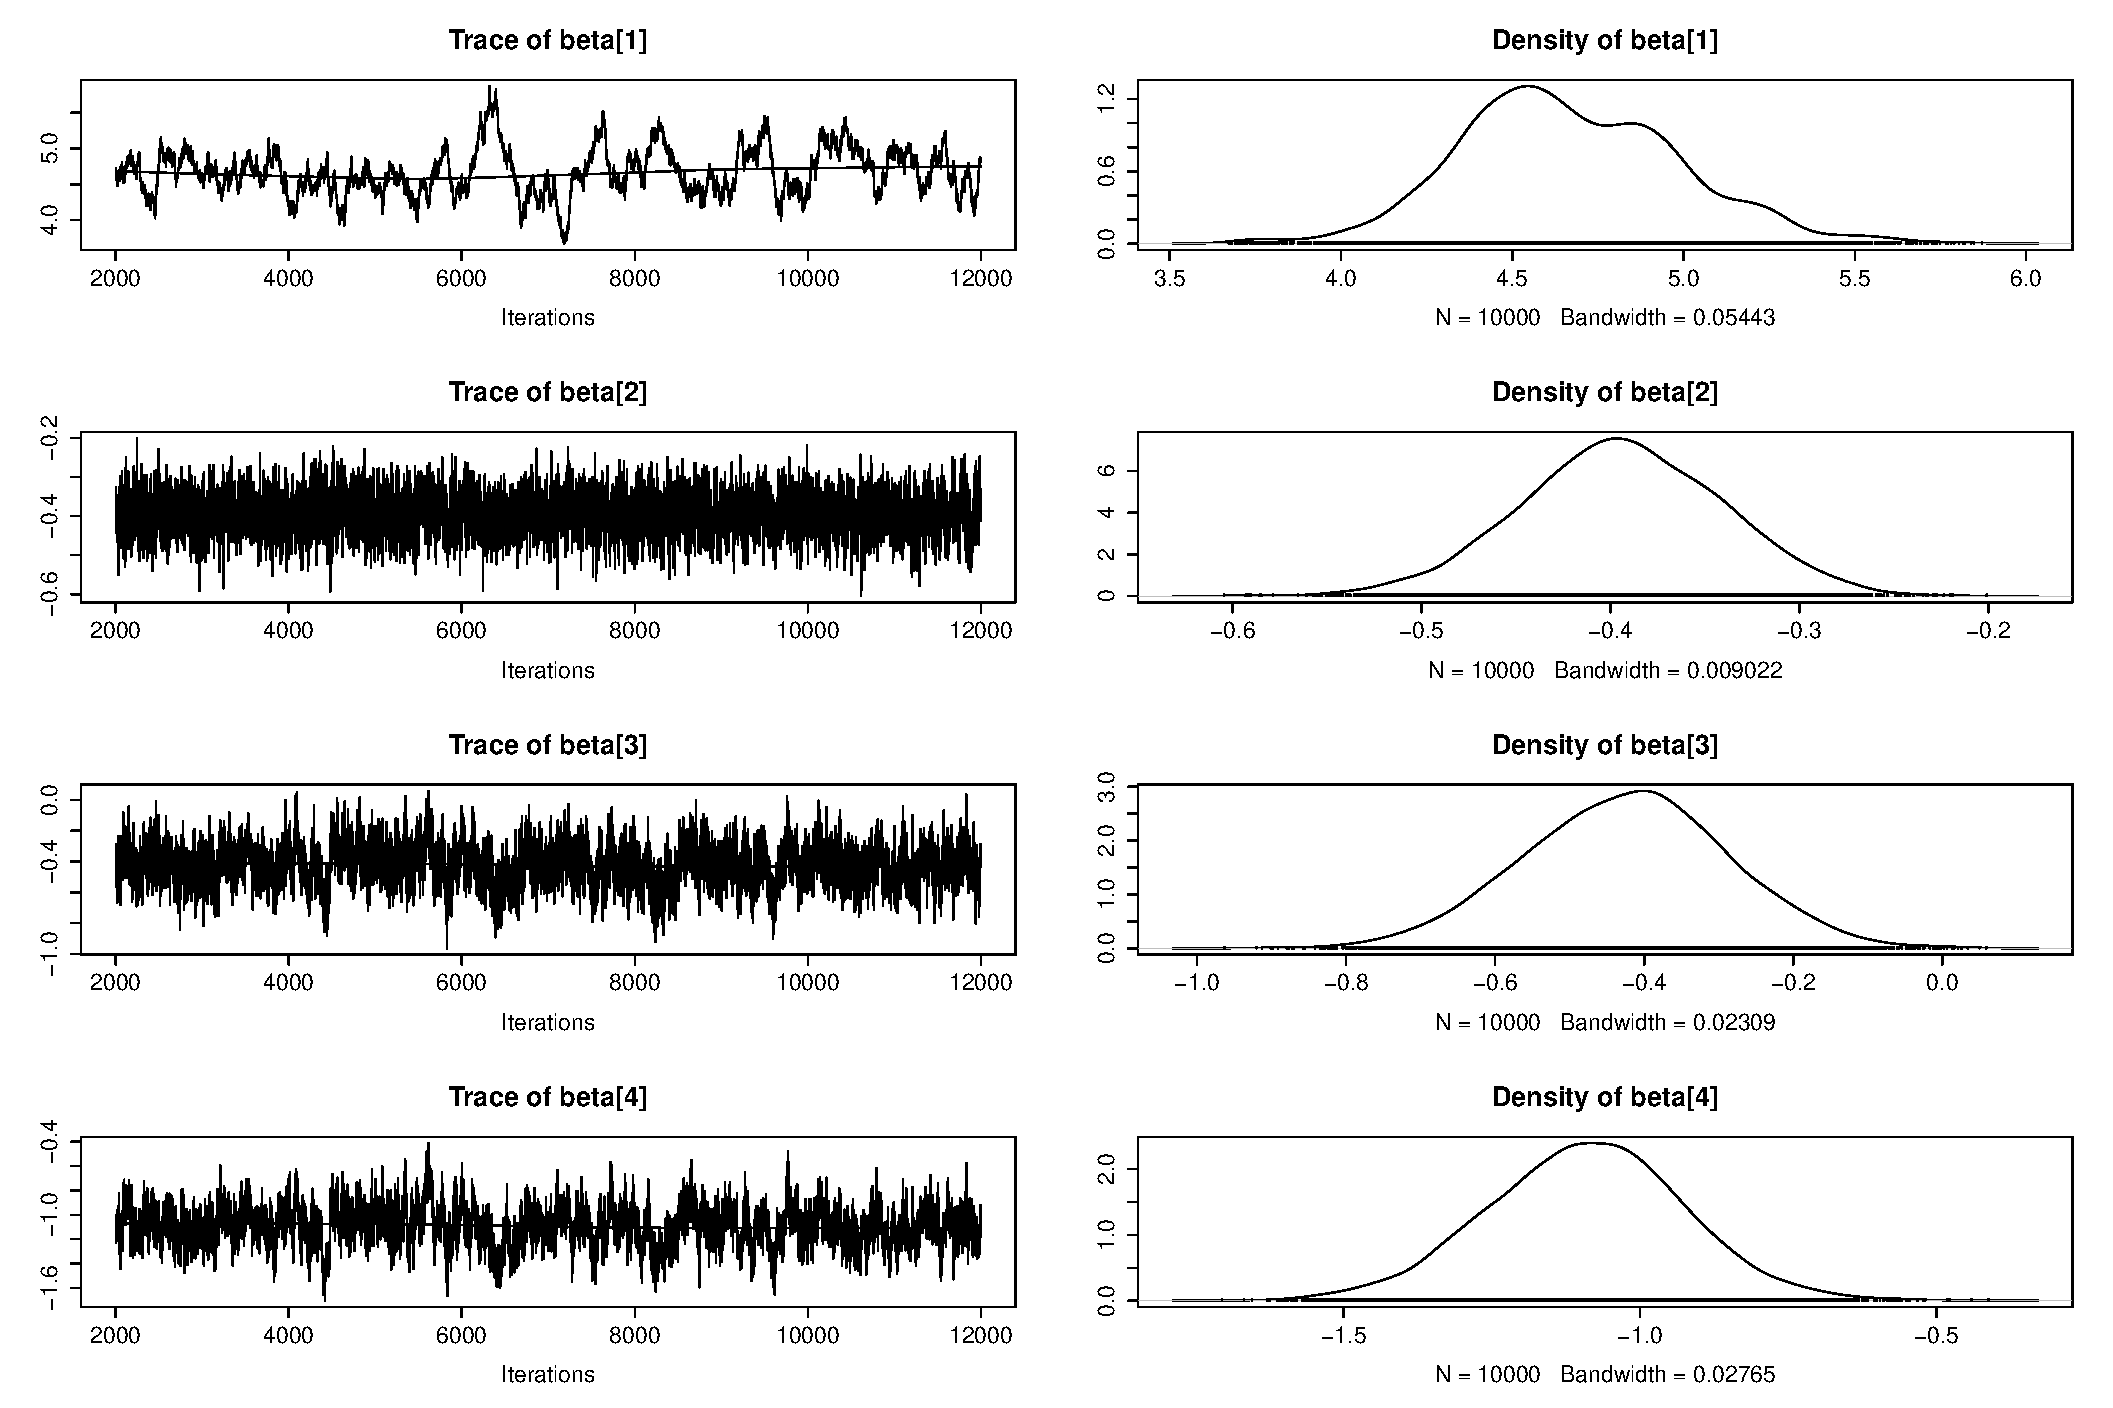
\includegraphics[width = 0.9\textwidth]{saturatedOutput/beta1-4.pdf}
\caption{Trace and density plots for the parameters $\beta_0, \beta_1, \beta_2$ and $\beta_3$.}
\label{saturated_beta1-4}
\end{figure}
\subsection{Model with Variable Selection}
The model can be improved upon by using a model that does variable selection and random effects with prior inclusion. This means that the model will no longer have all the variables which will give us a model which is less likely to over fit and will have less bias. The random effects means that the variable value is now changed with a variable probability where the probability comes from a normal distribution. The model string we used to incorporate this is
{\small
\begin{verbatim}
modelstring = "
model{
for(i in 1:n){
mean[i] = inprod(X[i,], beta)
y[i] ~ dnorm(mean[i],tau)
}
for (j in 1:p) {
ind[j] ~ dbern(pind)
betaT[j] ~ dnorm(0,taub)
beta[j] = ind[j]*betaT[j]
}
tau ~ dgamma(1, 0.001)
taub ~ dgamma(1, 0.001)
pind ~ dbeta(2,8)
}
"
\end{verbatim}
}
\begin{figure}[H]
\centering
	\begin{subfigure}[b]{0.49\textwidth}
		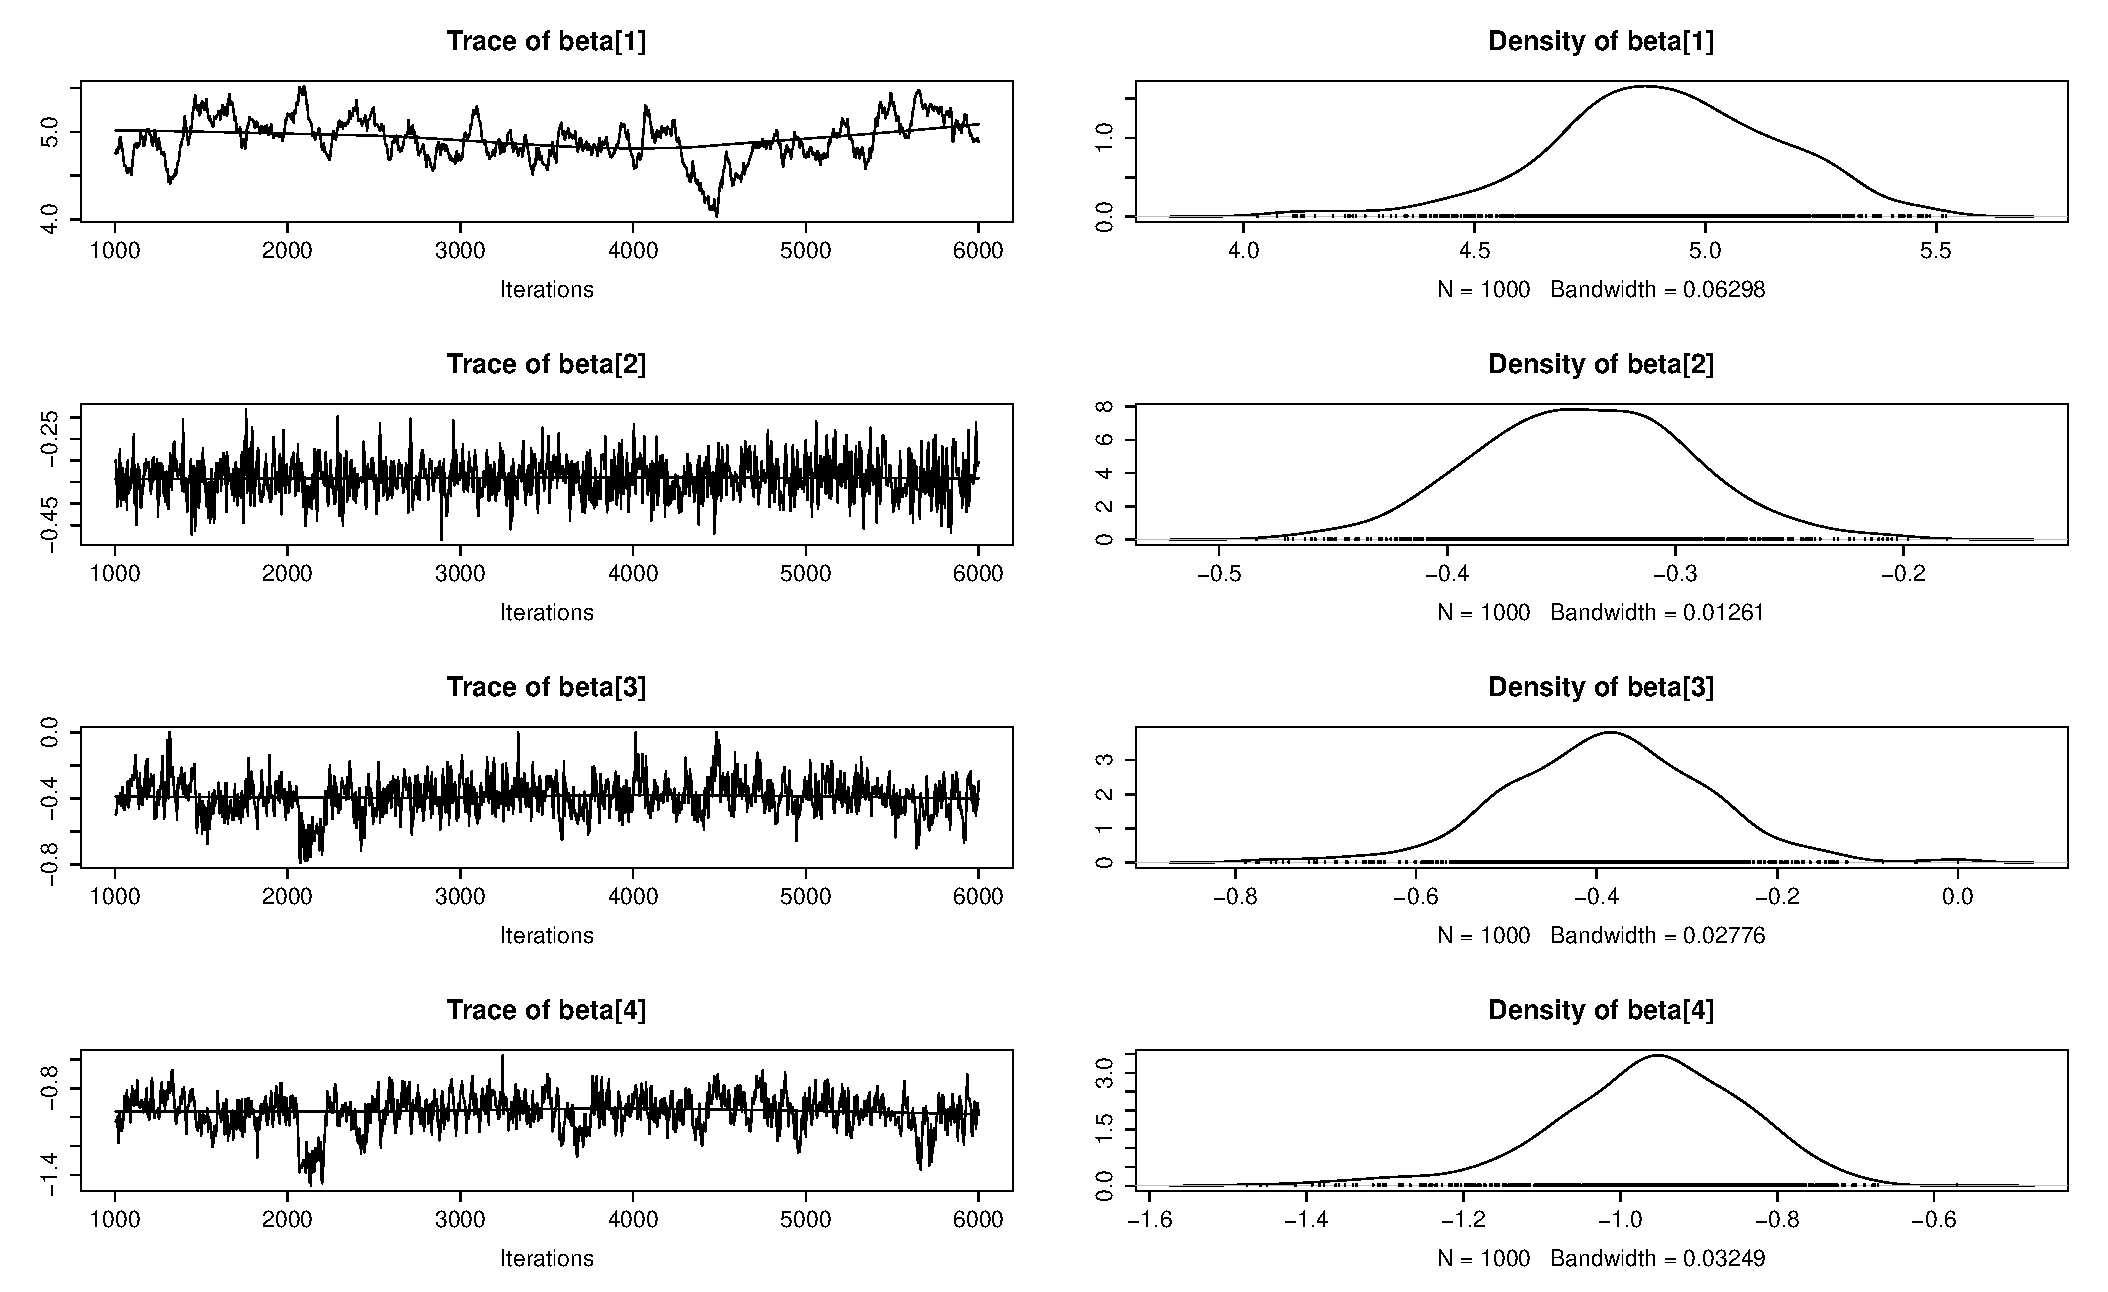
\includegraphics[width = \textwidth]{micePlot.pdf}
\caption{$\beta_0, \beta_1, \beta_2$ and $\beta_3$}
\label{micePlot}
	\end{subfigure}
	\begin{subfigure}[b]{0.49\textwidth}
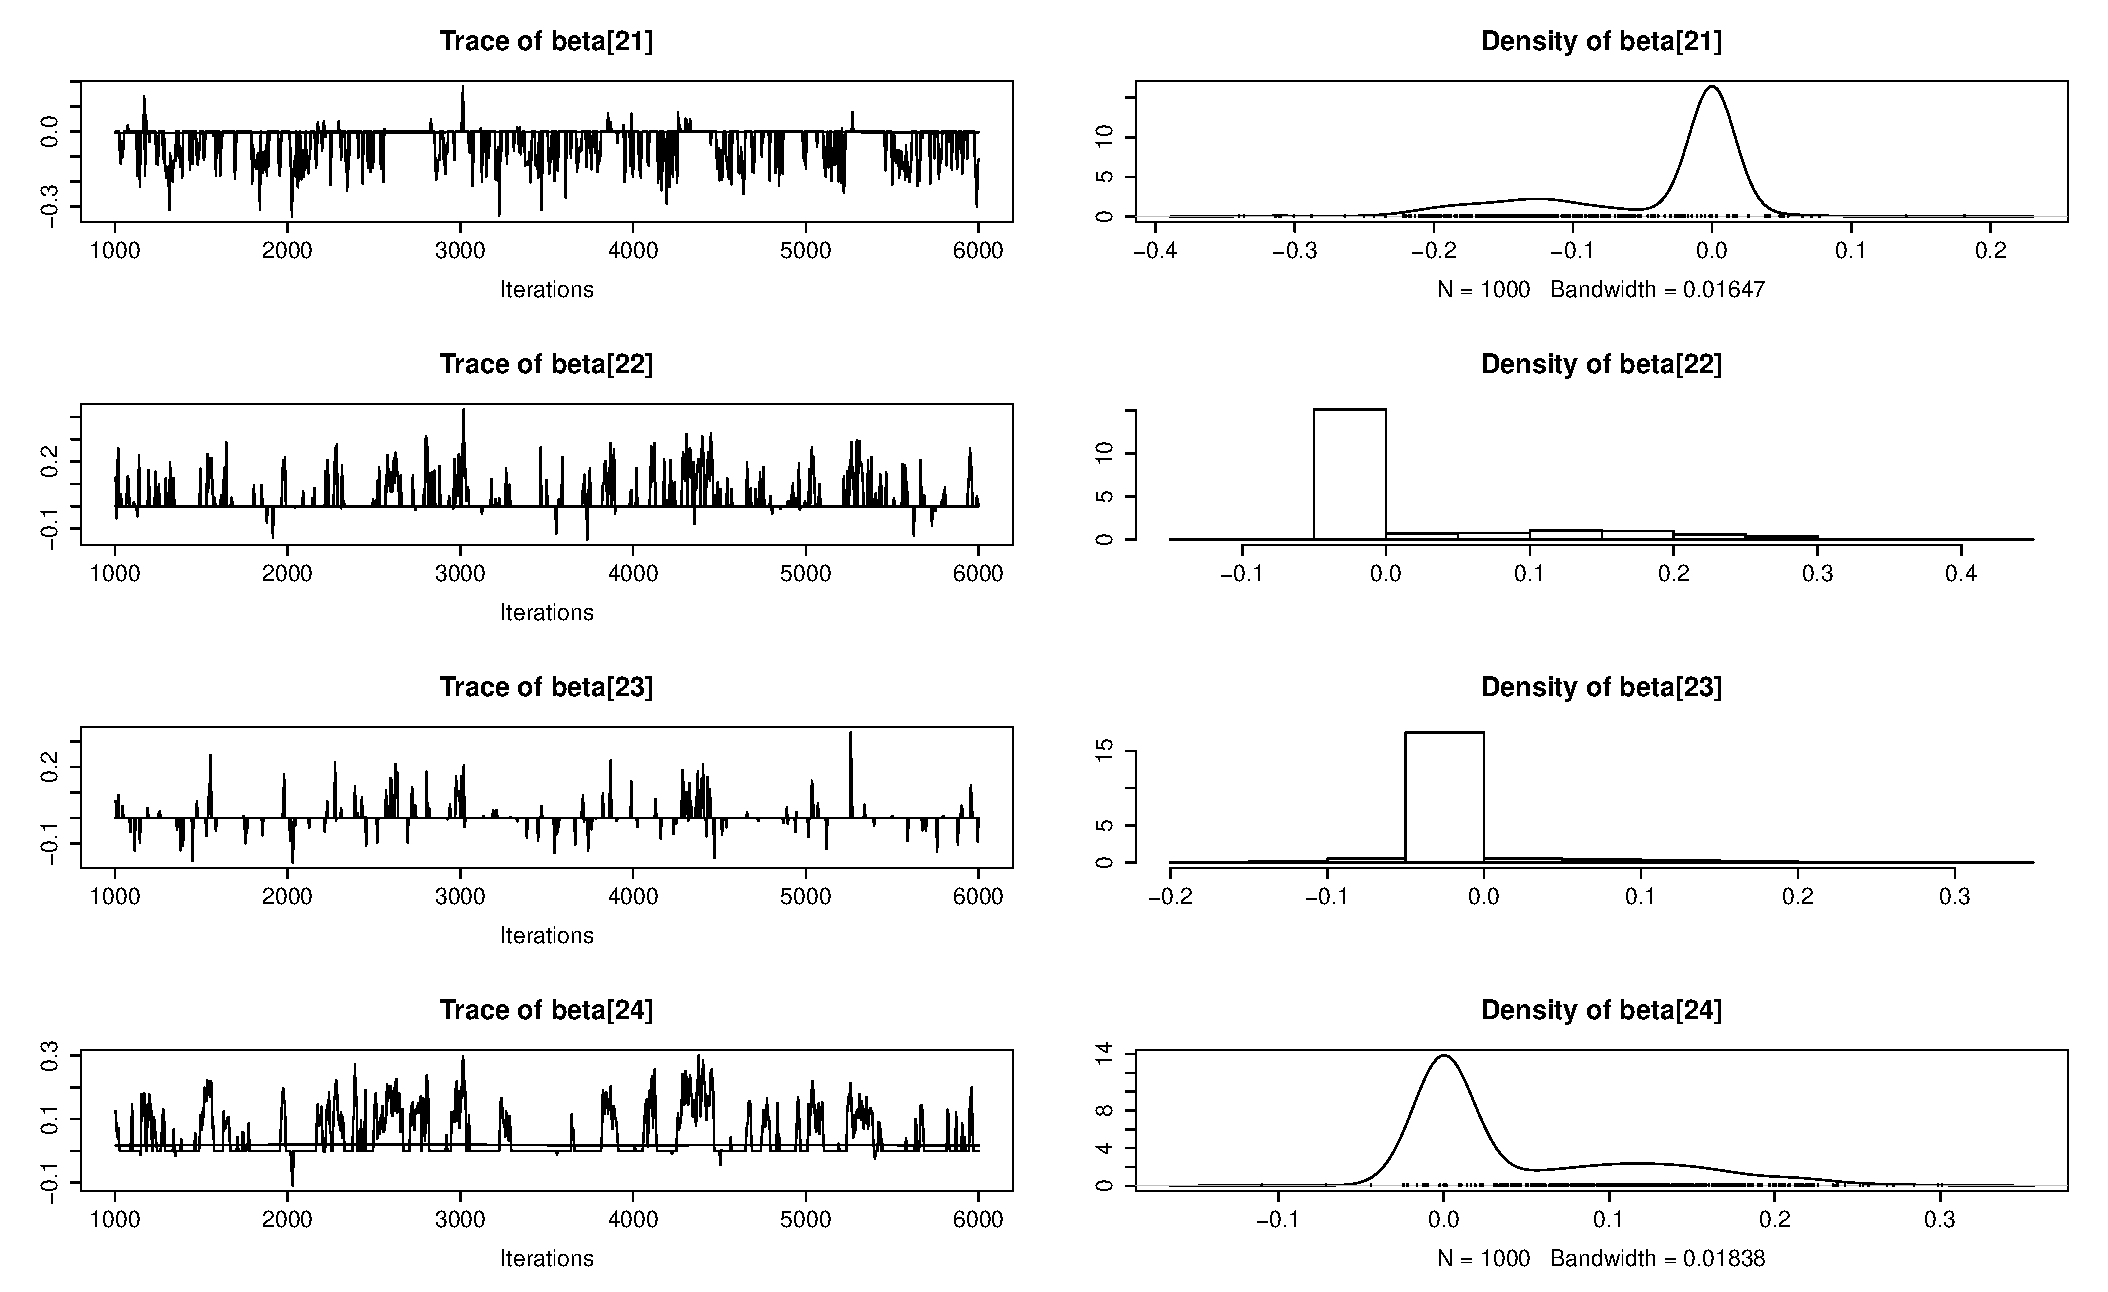
\includegraphics[width = \textwidth]{notIncludedBetas.pdf}
\caption{$\beta_{20}, \beta_{21}, \beta_{22}$ and $\beta_{23}$}
\label{notIncluded}
\end{subfigure}
\caption{Trace and density plots}
\end{figure}
\noindent We used this model to the data where the missing values had been replaced using the MICE method mention in Section~\ref{handling}. Since this is a better approach to modelling the data we ran the MCMC for a longer period of time. The burn is period is 1000 iterations and the run is 5000 iterations. As you can see in Figure~\ref{micePlot} the trace plot is now not as condensed because the JAGS model has included variable selection so some iterations give a value of 0. Figure~\ref{notIncluded} shows that the model has chosen for $\beta_{20}, \beta_{21}, \beta_{22}$ and $\beta_{23}$ to not be included in the model. This is shown by the trace plot regularly being 0 and in the density plots. The density plot for $\beta_21$ and $\beta_22$ are represented by histograms are there are so few values which are not approximately 0.
\\\\
The variable selection process has included some of the predictors. The \textsf{ind} vector can be though of as the probability that the corresponding predictor is in the model. Below we have the \textsf{R} output showing the mean \textsf{ind} values. We can see here that \textsf{ind[21] - ind[28]}, for example, have some uncertainty whether there respective variables should be in the model. The value for \textsf{ind[28]} has the lowest mean value and therefore the variable it corresponds to, \textsf{Householdu18}, is least likely to be in the model. 
\\\\
It is worth noticing that the variables \textsf{ind[21] - ind[28]}, representing Lived[2] - Lived[5], are potentially as low as they are because $10\%$ of the data corresponding to this, which is how long a person had lived in their house, was initially missing and therefore had be created during the MICE method.
{\small
\begin{verbatim}
ind[1]  ind[2]  ind[3]  ind[4]  ind[5]  ind[6]  ind[7]  ind[8]  ind[9] ind[10] ind[11]
1.000   1.000   0.991   1.000   1.000   1.000   1.000   0.999   1.000   1.000   1.000 
ind[12] ind[13] ind[14] ind[15] ind[16] ind[17] ind[18] ind[19] ind[20] ind[21] ind[22]   
1.000   1.000   1.000   1.000   1.000   1.000   1.000   1.000   1.000   0.286   0.256  
ind[23] ind[24] ind[25] ind[26] ind[27] ind[28] ind[29] ind[30] ind[31] ind[32] ind[33]
 0.164   0.374   0.983   0.211   0.473   0.096   1.000   1.000   0.611   1.000   1.000 
ind[34] ind[35] ind[36] ind[37] ind[38] ind[39] ind[40] ind[41] ind[42] ind[43] 
1.000   0.241   0.131   0.866   0.659   0.280   0.242   0.182   0.997   0.163 
\end{verbatim}
}
\section{Future Research}
A potential route to further the inferences in this paper would be be investigate and perform variable selection based on the correlations between the predictors within the data. This is discussed very briefly below.
\\\\
We can form the model matrix of the data providing we have converted the necessary predictors into factors. From this model matrix which contains only binary indicator variables we can form the correlation matrix. 

\begin{figure}[h!]
  \centering
    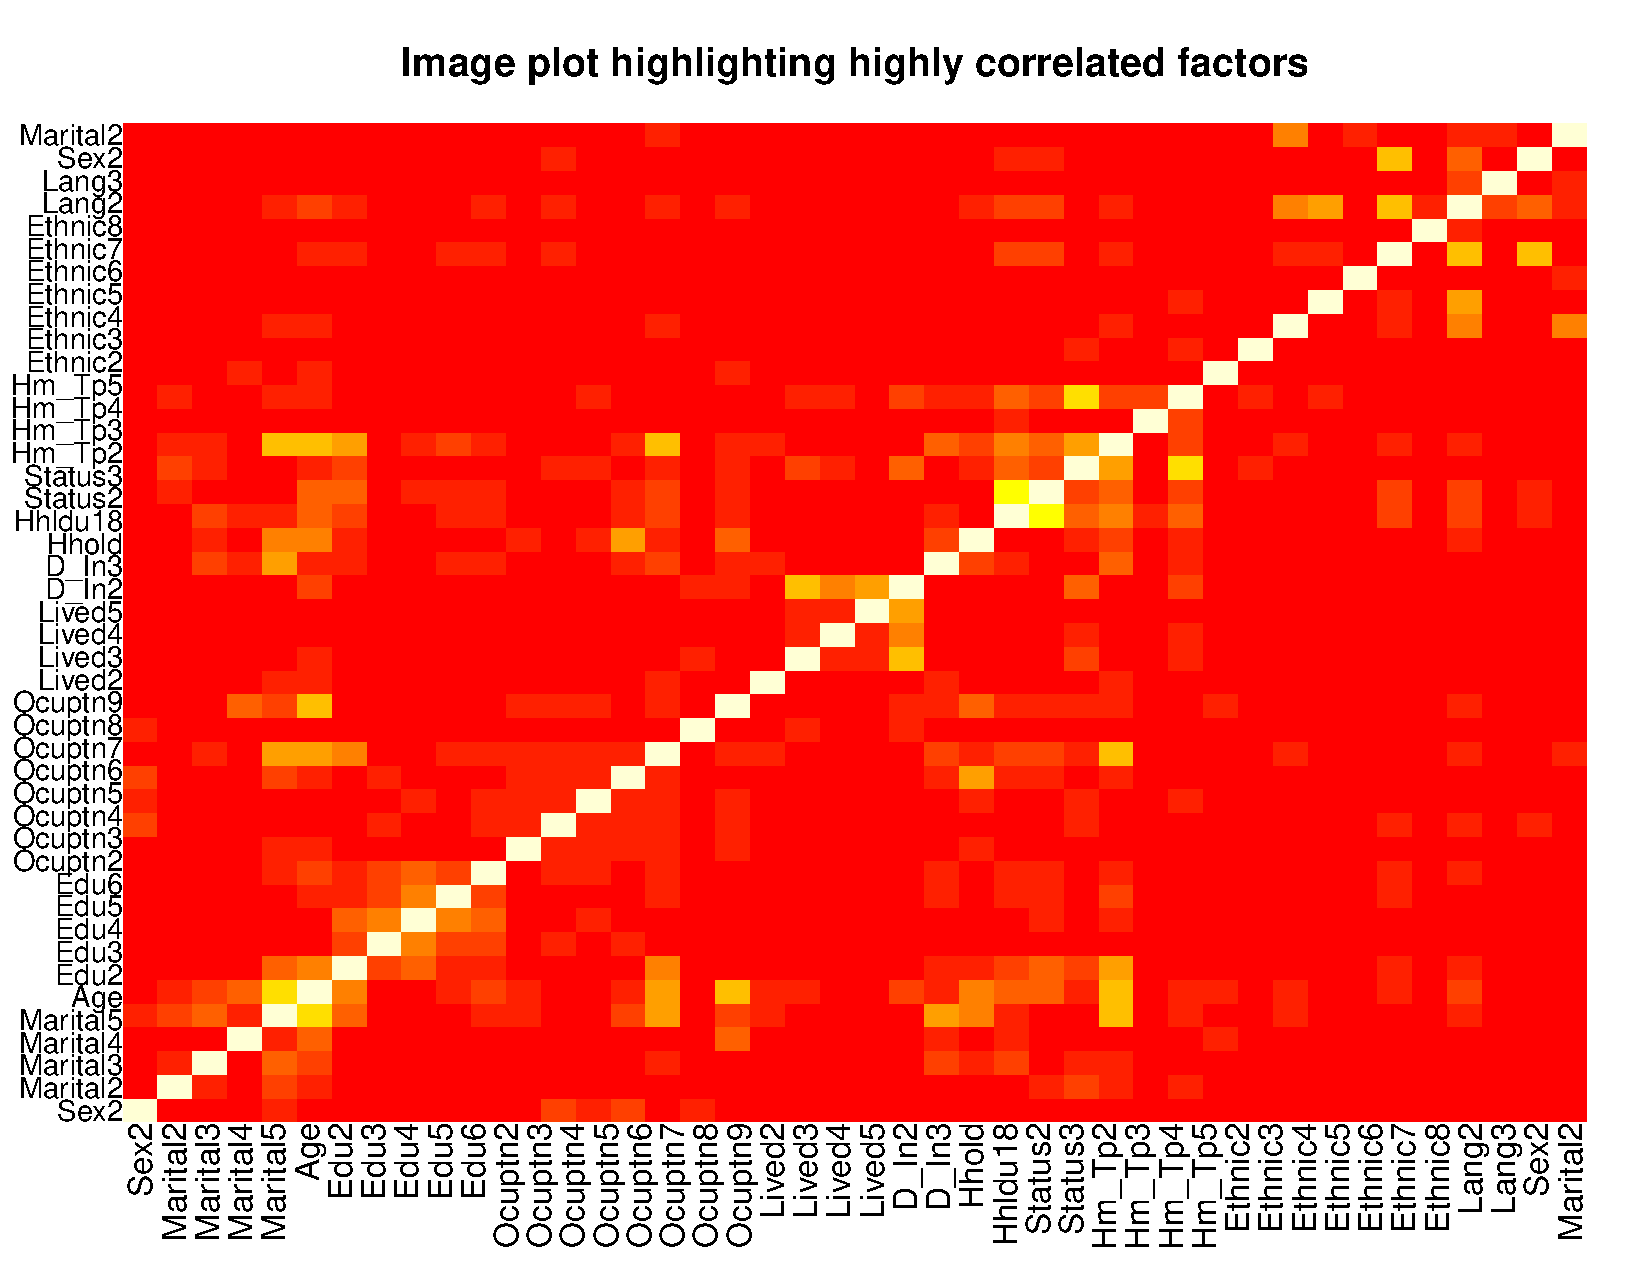
\includegraphics[width=0.72\textwidth]{FutureResearch/CorrImageNoThresh.pdf}
  \caption{Factors' correlation matrix.}
\end{figure}

\noindent This 42x42 matrix contains a lot of information pertaining to the marginal relations of every pair of levels of predictors in the model.
\\\\
We can add threshold to the matrix to only only highlight those pairs we deem to have a significant correlation, say an absolute value greater than 0.5. With this being a symmetric matrix it is sufficient to only inspect the those correlation which lie above the main diagonal. 
\begin{figure}[H]
  \centering
    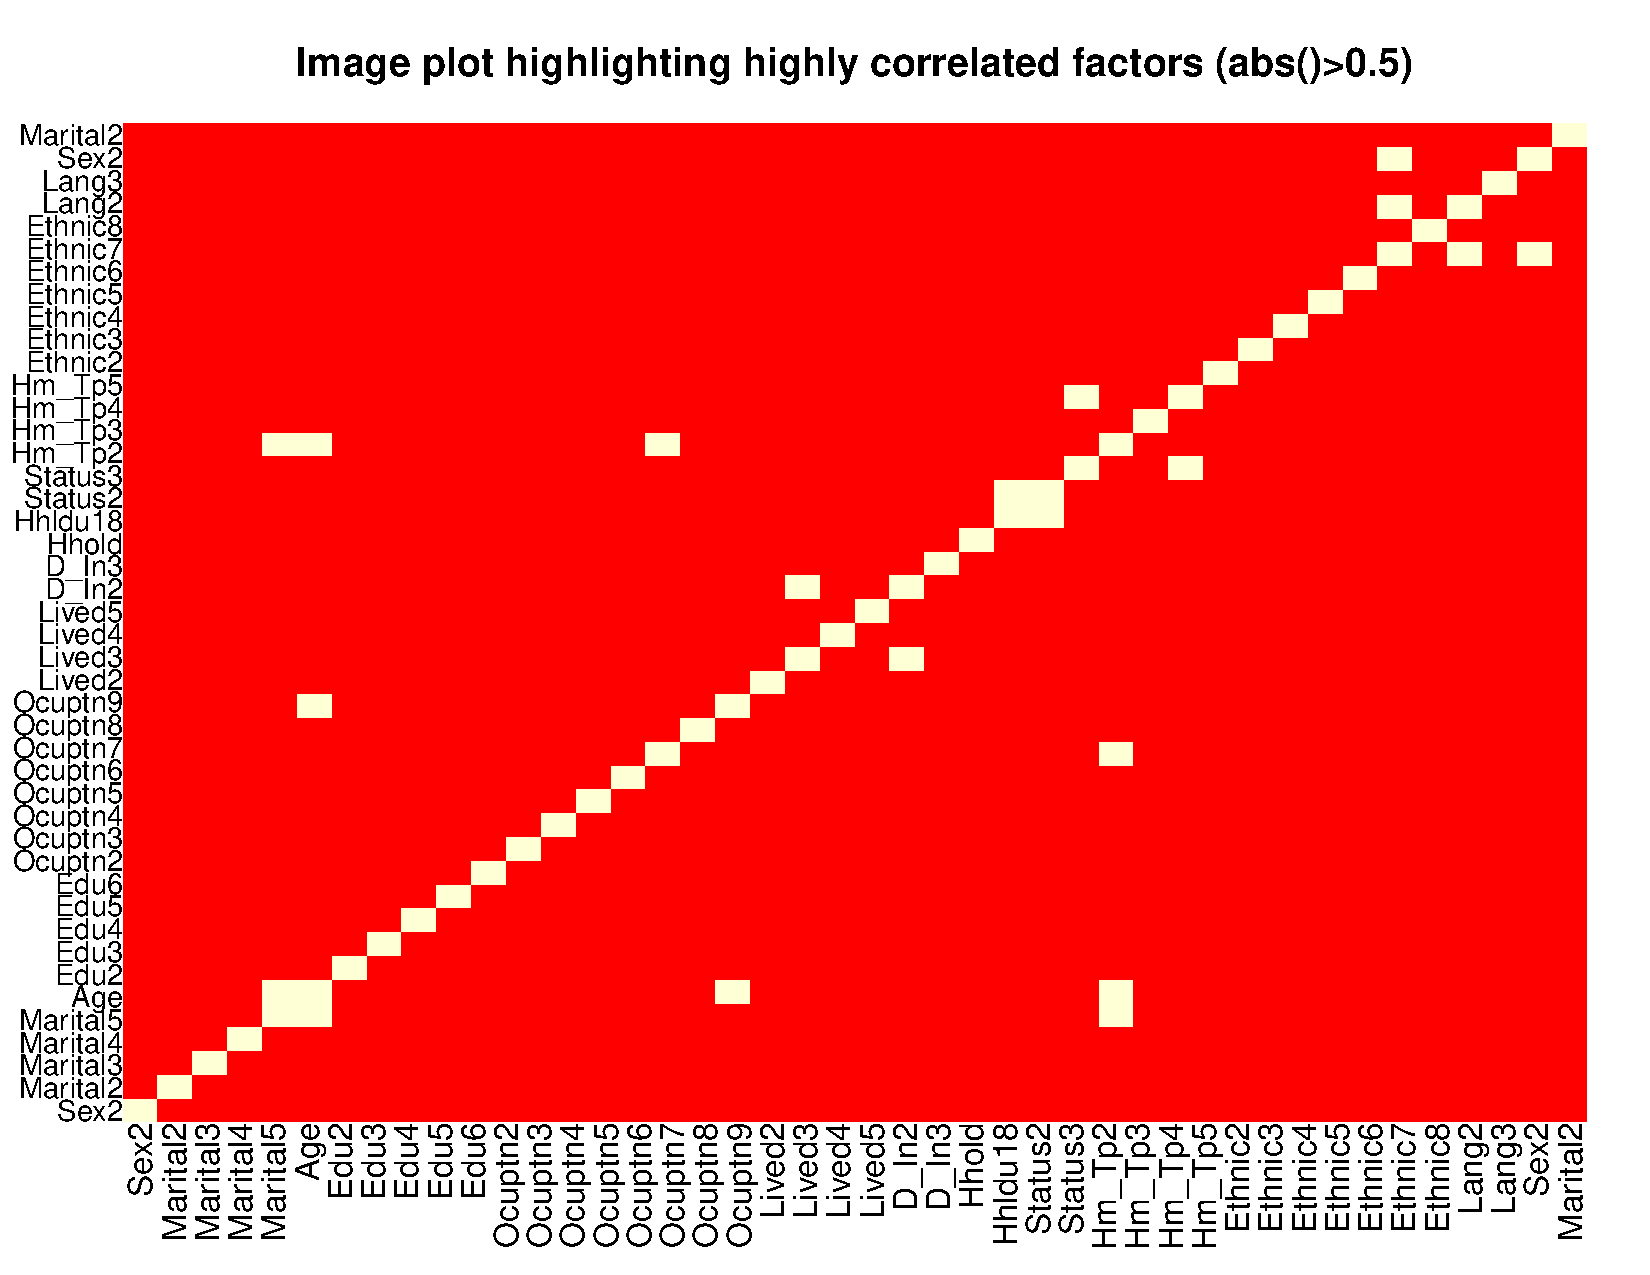
\includegraphics[width=0.72\textwidth]{FutureResearch/CorrImageWithThresh.pdf}
  \caption{Factors' correlation matrix with threshold.}
\end{figure}

\noindent From the plot below we see that there are ten such pairs of predictors. These high correlations could be used when deciding which predictors to include in a model.

\end{document}